\section{Donut Delivery Experiment: Creating and Selecting the Task Set} \label{sec:task_set}
A critical part of the Donut Delivery experiment was designing the right task set for participants to complete. In this section the rationale and approach to selecting the task set are discussed.

The size of the task set was based on two criteria. First, there needed to be enough tasks to get a good idea about performance. Second, the experiment was confined to be between 10-15 minutes based on the budget for the experiment, and also how long a participant could attend to tasks like this without losing interest and/or motivation. Using this criteria we decided to use around 40 tasks.

Experiment data was generated by creating random networks within the following bounds: $N = [8,35]$ (based on compute limitations), and $p_{trans}=[0.0,1.0]$ (as used in this formulation the transition probability indicates the probability that the UDT will actually move in a desired direction as opposed to one of the remaining undesired locations). All other parameters are as reported in \textbf{insert citation in final version}. The starting position of the unmanned delivery truck (UDT) and the motorcycle gang (MG), and delivery destination were randomly selected from the available nodes (i.e. road intersections).

Each road network was created by randomly selecting a value for N in the given range, then uniformly randomly selecting a method from 1) \emph{Watts-Strogatz}\footnote{See \url{https://en.wikipedia.org/wiki/Watts-Strogatz_model}} ; 2) \emph{expected degree}\footnote{See \cite{Chung2002-jh}} where the expected degree was a Normal distribution with mean 4 and standard deviation 1; 3) \emph{Erd\"{o}s-R\`{e}yni}\footnote{See \url{https://en.wikipedia.org/wiki/Erdős–Rényi_model}} specifying N and E (number of edges) with $E = 2$; and 4) \emph{static scale free}\footnote{See \url{https://en.wikipedia.org/wiki/Scale-free_network}} with $E = 2$ and $\alpha_{out}=2$. All graphs were required to be fully connected. A total of 500 networks were generated using this method, and \xQ{} and \xO{} were calculated for each one. Figure~\ref{fig:appendix_exp_data} shows the full data set on the top. A subset of those networks were chosen for the final experiment task set.

A more detailed explanation of Fig.~\ref{fig:appendix_tot_set} is merited. In this figure 341 of the 500 generated networks are represented---the other 159 networks were excluded due to the edge-to-node ratio being `too high' (i.e. greater than 2.5, making the networks difficult to process because of the density of edges), the distance to the delivery destination being `too close' (i.e. the delivery truck being right next to the exit), or the distance to the motorcycle gang being `too  close' (i.e. the truck starting right next to the motorcycle gang). They are plotted in a scatter plot only based on their \xQ{} and \xO{} values (e.g. differing values of $N$, $p_{trans}$, starting location, et cetera are not depicted). Blue dots represent a `successful' delivery (i.e. final reward greater than or equal to 0) and the orange dots represent a `failed' delivery (final reward less than zero). In order to emphasize, each colored dot represents the outcome of a draw from the \pri{} reward distribution of a single road network problem ($N$ and $p_{trans}$, UDT starting location, MG starting location, and delivery destination, see \textbf{[OMITTED FOR ANONYMITY]} for more detail), that was solved by 1000 iterations of a Monte-Carlo Tree Search (MCTS) solver with depth 3, and exploration constant 1000. The presence of blue dots in the bottom left corner of the plot indicates unlikely, or `lucky', successes (see Figures~\ref{fig:appendix_lucky} and \ref{fig:appendix_unlucky}). It is interesting to point out that this plot \emph{did not exist} while we were designing \xQ{} and \xO{}, this plot was made only \emph{after} \xQ{} and \xO{} were designed. The fact that the density of successes is higher when both \xQ{} and \xO{} are `high' is an indicator that they are in fact performing their function.

\begin{figure}[tbp]
    \centering
    \begin{subfigure}[b]{0.80\linewidth}
        \centering
        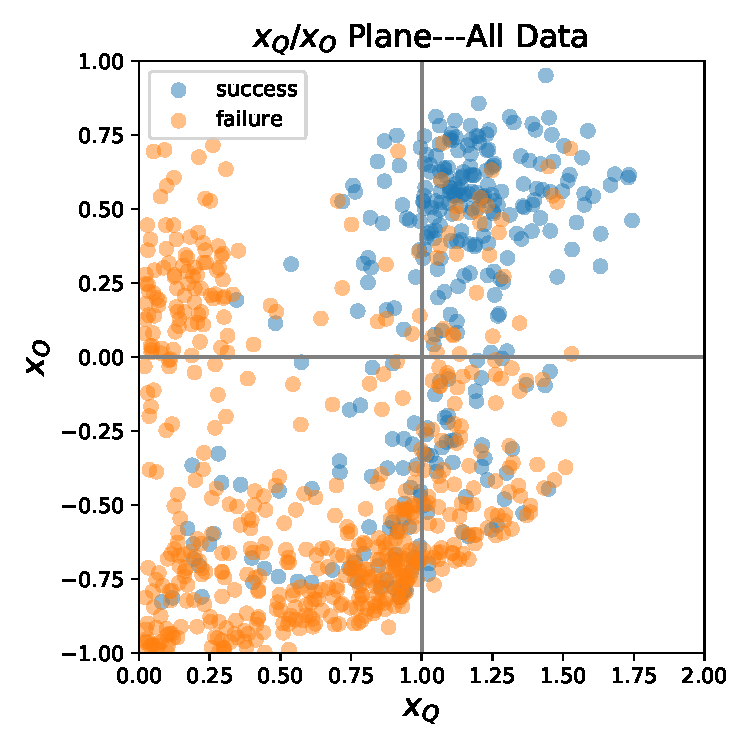
\includegraphics[width=0.95\linewidth]{Figures/xQxO_Plane.pdf}
        \vfill
        \caption{Total set of generated networks}
        \label{fig:appendix_tot_set}
    \end{subfigure}%
    \\
    % \hfill
    \begin{subfigure}[b]{0.80\linewidth}
        \centering
        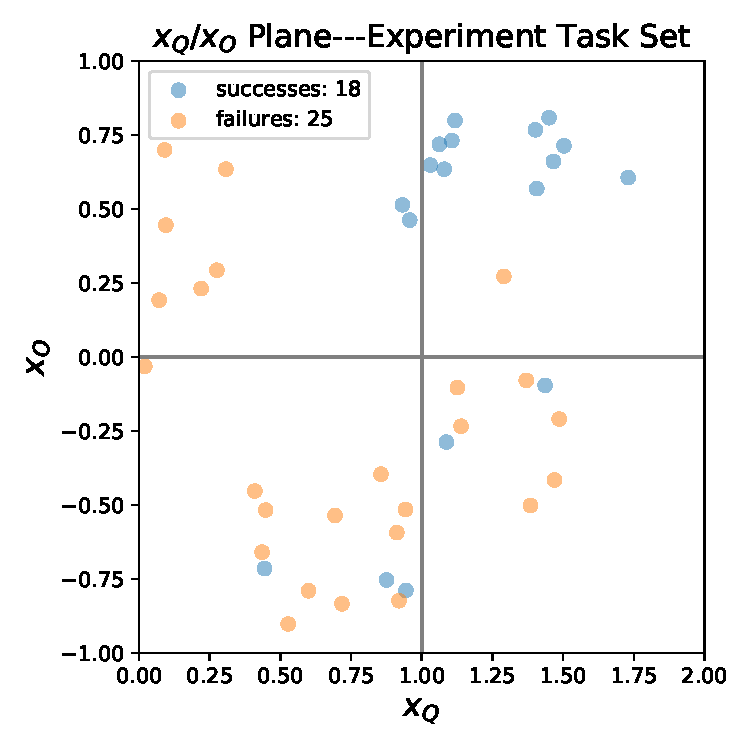
\includegraphics[width=0.95\linewidth]{Figures/xQxO_plane_experiment_set.pdf}
        \caption{Subset of networks used in the MTurk experiment}
        \label{fig:appendix_exp_set}
    \end{subfigure} 
    \caption{Generated Road Networks and Final Experiment Task Set}
    \label{fig:appendix_exp_data}
    \vspace{-0.2cm}
\end{figure}

\begin{figure}[tbp]
    \centering
    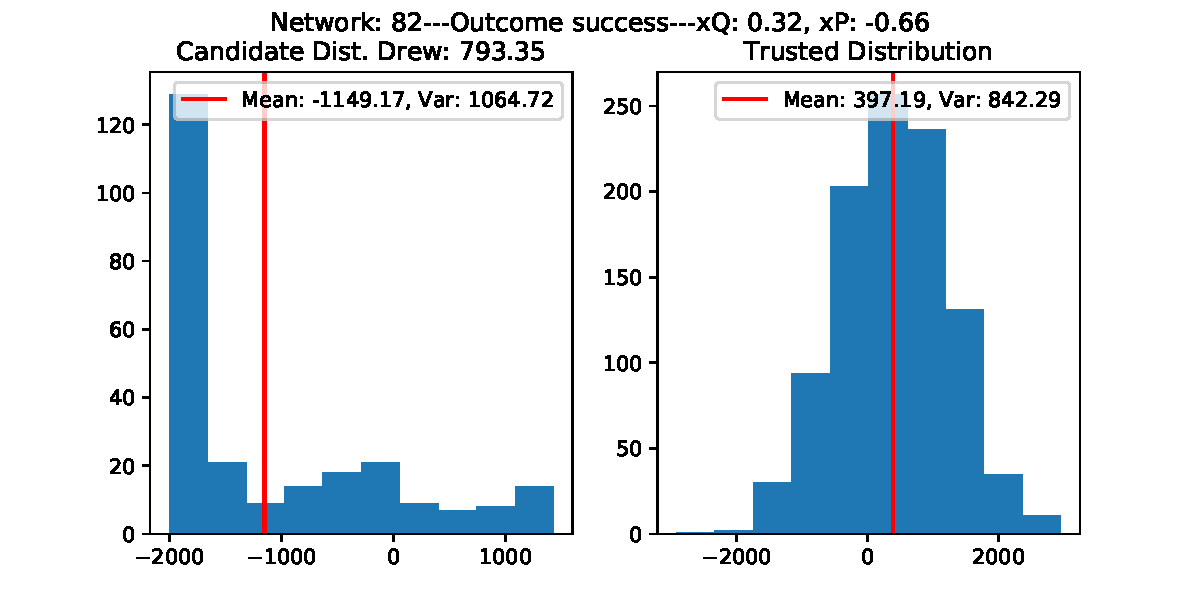
\includegraphics[width=1.0\linewidth]{Figures/mturk_5_Ntprob_solver_82_surprisesuccess.pdf}
    \vfill
    \caption{Example of a case in which the policy was `lucky' during a simulation run. (Right) histogram of `Trusted' reward distribution. (Left) Histogram of `Candidate' rewards distribution. In this case the simulation drew an outcome with $\ri = 793.35$ resulting in a successful delivery.}
    \label{fig:appendix_lucky}
\end{figure}

\begin{figure}[tbp]
    \centering
    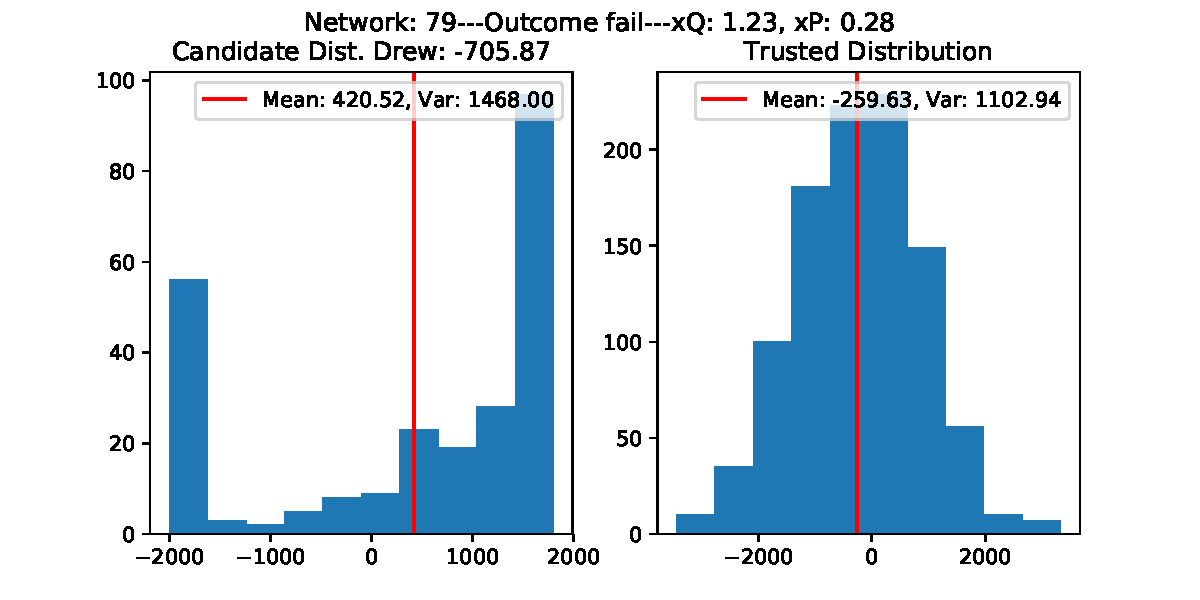
\includegraphics[width=1.0\linewidth]{Figures/mturk_5_Ntprob_solver_79_surprisefail.pdf}
    \vfill
    \caption{Example of a case in which the policy was `unlucky' during a simulation run. (Right) histogram of `Trusted' reward distribution. (Left) Histogram of `Candidate' rewards distribution. In this case the simulation drew an outcome with $\ri = -705.87$ resulting in an unsuccessful delivery.}
    \label{fig:appendix_unlucky}
\end{figure}

In order to understand the effects that the two \famsec{} factors had over the entire \xQ{}/\xO{} space, we selected the 43 examples from the full data set by splitting the space into a grid and then proportionally selecting networks based on success and failure. First the data was split in quadrants and the total number of networks from each quadrant was selected based on the proportion of networks in the quadrant (here quadrants start at $1$ in the top right corner, $2$ in the top left, and so on continuing counter-clockwise).

For each quadrant the task set networks were selected using the following procedure after calculating the total number of examples from each quadrant: 1)Calculate the proportion of successes to failures in each quadrant, and use that to choose how many success and failures should be drawn from each quadrant (see Tab.~\ref{tab:q_table} for the actual numbers); 2) draw that number of successes and failures in a way such that they are \emph{spread out} and not clustered near to each other (i.e. using an approach like Latin Hypercube sampling). The final set of networks used in the experiment is plotted in Fig.~\ref{fig:appendix_exp_set}, and Table~\ref{tab:q_table} shows the breakdown of the numbers by quadrant. Generally, the proportions from each quadrant were reasonably near to the proportions of those in the original data set from Fig.~\ref{fig:appendix_tot_set}; one stand-out example is the number of examples from the third quadrant that initially contained $43\%$ of all networks, in the experiment set only $35\%$ of the networks are in experiment 3. This limit was introduced on purpose so no single quadrant would dominate the number of experiment tasks.

Ultimately, we believe that the approach presented here is a principled way to have drawn the experiment examples that faithfully reflects the actual distribution of networks in the full data set, while also taking precautions to represent the full extent of the networks in the \xQ/\xO{} space, and fit within the limitations of time imposed because of the budget and the capability of participants to stay focused on a task like this.

\begin{table}
    \centering
    \caption{Breakdown of the original dataset and the smaller task-set used in the MTurk experiment}
    \label{tab:q_table}
    \begin{tabular}{r|ccccc}
\toprule
             & Total & Quad. 1 & Quad. 2 & Quad. 3 & Quad. 4 \\ \hline
           N &    43 &      12 &       8 &      15 &       8 \\
  Proportion & 1.000 &   0.229 &   0.180 &   0.434 &   0.156 \\
   Successes &    18 &      11 &       2 &       3 &       2 \\
    Failures &    25 &       1 &       6 &      12 &       6 \\
Success/Fail &    -- &   9.714 &   0.283 &   0.214 &   0.417 \\
\bottomrule
\end{tabular}
\end{table}
